\chapterimage{chapter_head_2.pdf} % Chapter heading image

\chapter{Princípios elementares na dança de salão}

Antes de iniciar as explicações no capítulo, 
é necessário partir desde uma linguagem comum;
com este propósito, 
significados de algumas palavras bem definidas na literatura são mostrados a continuação:
 
\begin{definition}[Princípio:] 
\index{Princípios}
\label{def:Principio}O Dicionário Priberam da Língua Portuguesa \cite{priberamprincipio} define princípio como:
Frase ou raciocínio que é base de uma arte, de uma ciência ou de uma teoria.
Adicionalmente o Dicionário Online de Português, DICIO \cite{dicioprincipio}, define princípio como:
Informação básica e necessária que fundamenta uma seção de conhecimentos.
Exemplo:princípios da matemática.
\end{definition}

\begin{definition}[Casal:] 
\index{Casal}
\label{def:Casal} O Dicionário Priberam da Língua Portuguesa \cite{priberamcasal} define casal como:
Par formado por um macho e uma fêmea.
Exemplo: casal de cavalos, casal de pombas, casal de humanos.
\end{definition}

\begin{definition}[Par:] 
\index{Par}
\label{def:Par} O Dicionário Priberam da Língua Portuguesa \cite{priberampar} define par como:
Igual, semelhante, parceiro.
Cada uma das pessoas que constituem uma dupla na dança.
\end{definition}


Usando como base os significados mostrados anteriormente, 
serão descritos alguns termos muito utilizados na dança\footnote{
Para as definições, foi priorizado o uso da palavra par sobre a palavra casal,
para poder definir às entidades dançantes independentemente do sexo dos participantes.}.
Assim,  são propostas as seguintes definições:

\begin{definition}[Paradigma da condução (Dança):] 
\index{Condução} 
\label{def:ParadigmaConducao} 
Este é um modelo de dança a dois usado na \hyperref[def:DancaSalao]{\textbf{dança de salão}},
\hyperref[def:DancaSocial]{\textbf{dança social}}, etc. 
E indica que entre as pessoas que conformam a dança, 
existe uma transmissão de informação relativa à movimentação e as pausas, no \hyperref[def:Par]{\textbf{par}} dançante; 
de modo que, a informação tem um fluxo unidirecional no médio de transmissão,
que vá desde o \hyperref[def:Condutor]{\textbf{condutor}} ate o \hyperref[def:Seguidor]{\textbf{seguidor}}. 
\end{definition}
\index{Condutor} 

\begin{definition}[Condutor (Dança):] 
\index{Condutor} 
\label{def:Condutor} 
A pessoa que tem o papel de conduzir ou propor o movimento ao \hyperref[def:Seguidor]{\textbf{seguidor}}. 
O objetivo técnico das pessoas que optam por este rol na dança, é chegar 
a ter a sensibilidade necessária para entender onde está localizado espacialmente, 
e como distribui o peso do corpo, o \hyperref[def:Seguidor]{\textbf{seguidor}}; 
de modo que seja possível para o condutor aplicar sobre o \hyperref[def:Seguidor]{\textbf{seguidor}}, 
uma mistura de indicações, forças e torções,  
para provocar os movimentos ou pausas desejadas;
chama-se a isto saber conduzir.
Sinônimos de condutor: Líder (Dança).
\end{definition}

\begin{definition}[Seguidor (Dança):] 
\index{Seguidor} 
\index{Conduzido} 
\label{def:Seguidor} 
A pessoa que recebe a condução e proporciona uma resposta corporal. 
O objetivo técnico das pessoas que optam por este rol na dança, é chegar 
a ter a sensibilidade necessária para entender e incorporar as conduções,
independentemente de quem seja a pessoa que aplique a condução;
chama-se a isto ser conduzível.
Sinônimos de seguidor: \textbf{Conduzido}.
\end{definition}

\PRLsep{Tipos de abraço nas danças a dois}

\begin{definition}[Abraço de dança:]
\index{Abraço de dança}
\label{def:abracodedanca}  
É um abraço onde o \hyperref[def:Condutor]{\textbf{condutor}} 
rodeia com a mão direta as costas do \hyperref[def:Seguidor]{\textbf{seguidor}},
numa linha meia entre a linha dos ombros e a linha da parte baixa do tórax;
enquanto a mão esquerda, do condutor, segura com o braço semi flexionado a mão direita do seguidor,
colocando ambas mãos a altura do ombro da pessoa mais baixa do \hyperref[def:Par]{\textbf{par}}.
Por outro lado, o seguidor também rodeia com seus braços ao condutor,
de modo que seu braço esquerdo rodeie o braço direto do condutor ate chegar,
na medida do possível, na altura dos ombros; 
é preferível que a palma da mão esquerda do seguidor não esteja apontando ao chão,
para evitar que inconscientemente o seguidor recarregue seu peso no ombro do condutor,
pelo que uma alternativa seria que a palma da mão do seguidor aponte algum ponto do próprio seguidor.
Por motivos similares, é preferível que o cotovelo do braço direito do seguidor,
que segura a mão do condutor,
não aponte ao chão e sim e sim que esteja ligeiramente levantado,
para não seja esquecido que o peso desse braço ou do corpo não deve ser recarregado no condutor. 



Em samba de gafieira comumente nos encontraremos num abraço de dança:
\begin{itemize}
\item Com os pés na postura de X, ou
\item Com os pés e o corpo frente a frente om seu par, é dizer uma postura frente a frente.
\end{itemize}
\end{definition}


\begin{definition}[Firmeza de braços (Dança):]
\index{Firmeza de braços}
\label{def:brazosfirmes} 
Que o \hyperref[def:Condutor]{\textbf{condutor}} e \hyperref[def:Seguidor]{\textbf{seguidor}}
tenham os braços firmes, não implica fazer força pra submeter ao par;
e sim, ativar os músculos o mínimo e necessário para manter a posição relativa e postura dos braços.
de modo que a informação de condução passe a traves dos braços e chegue, com fidelidade, ao corpo do seguidor.

Outra forma de descrever a firmeza dos braços, 
é indicando que esta ação implica ter uma ativação muscular e auto controle, 
para suprimir conscientemente alguns graus de liberdade que existem nas articulações nos braços, 
dependendo da situação e do estilo de dança.
Alguns destes graus de liberdade são obtidos devido a:
\begin{itemize}
\item O movimento de flexão no pulso,
\item movimento de rotação no antebraço,
\item movimento de flexão no cotovelo,
\item movimentos de rotação e abertura no ombro.
\end{itemize}
\end{definition}

\PRLsep{Tipos de danças a dois}

Para finalizar as definições neste capítulo, foram tomados dois conceitos do artigo,
``Conceitos e definição de Dança de Salão'' \cite{Zamoner2012};
e modificações foram feitas para adaptar as definições aos conceitos de \hyperref[def:Condutor]{\textbf{condutor}} e \hyperref[def:Seguidor]{\textbf{seguidor}}, usados ao longo deste livro.

\begin{definition}[Dança social:]
\index{Dança social} 
\label{def:DancaSocial} 
É uma dança com fim recreativo de prática social, não cênica, nem competitiva, 
que não tem um interesse artístico, histórico, geográfico ou técnico; 
que se universaliza e consiste na movimentação dos corpos do \hyperref[def:Par]{\textbf{par}} de dança  \cite{Zamoner2012}, 
onde existe o rol do \hyperref[def:Condutor]{\textbf{condutor}} 
e do \hyperref[def:Seguidor]{\textbf{seguidor}} (papeis intercambiáveis), 
ate onde o nível técnico do par o permita.
\end{definition}

\begin{definition}[Dança de salão:]
\index{Dança de salão}
\label{def:DancaSalao}  
É uma arte que procura conservar suas características técnicas, 
sua origem histórica e geográfica, e se universaliza em práticas sociais. 
Esta arte consiste na interpretação improvisada da música por médio dos movimentos 
dos corpos de um \hyperref[def:Par]{\textbf{par}} de dança \cite{Zamoner2012}, 
utilizando o \hyperref[def:ParadigmaConducao]{\textbf{paradigma da condução}} .
\end{definition}


%%%%%%%%%%%%%%%%%%%%%%%%%%%%%%%%%%%%%%%%%%%%%%%%%%%%%%%%%%%%%%%%%%%%%%%%%%%%%%%%
\section{Princípios elementares e gerais na dança de salão}
\label{sec:PrincipioGeral}
\index{Princípios elementares!Dança de salão}


\begin{tcbattention}
É importante aclarar
que os princípios elementares expostos neste capítulo e posteriores, 
não estão regulamentadas por nenhuma entidade ou instituição; assim, 
estes princípios refletem, o meu aprendizado de distintos professores,
interpretações pessoais  e deduções. 
\end{tcbattention}

Neste capítulo veremos um conjunto de \hyperref[def:Principio]{\textbf{princípios elementares}}, 
e a explicação de como o cumprimento ou não destes, 
afetam ao desenvolvimento estético e técnico da \hyperref[def:DancaSalao]{\textbf{dança de 
salão}}\footnote{Ou na \hyperref[def:DancaSocial]{\textbf{dança social}} sim se está interessado em levar estas ideias a esse âmbito.}  no \hyperref[def:ParadigmaConducao]{\textbf{paradigma da condução}}.

Os \hyperref[def:Principio]{\textbf{princípios elementares}} que veremos neste capítulo não devem ser
tratados como leis, e sim como diretrizes a serem usadas como padrão de inicialização, de modo que 
os dançarinos analisarão cada caso e se necessário criarão uma exceção e atuarão conforme ela.

Serão usados neste capítulo termos como \hyperref[def:Condutor]{\textbf{condutor}} e \hyperref[def:Seguidor]{\textbf{seguidor}}; 
mas, não existe nenhuma obrigatoriedade ou restrição para as pessoas, 
na escolha de algum destes papéis na dança.
Porem, é comum ver que o papel de condutor é escolhido tradicionalmente pelos homens e o papel de seguidor pelas mulheres.
%só são um recurso literário para o melhor entendimento das explicações mostradas aqui.

A continuação são listadas alguns princípios elementares e gerais na dança de salão, 
que abrangem um conjunto amplo de estilos de dança.\\

\begin{description}

\item[Rodar o salão:] Que os dançarinos executem sua dança se deslocando circularmente no salão, 
é importante para criar a ilusão de que o espaço de dança é maior, dado que mesmo
tendo uma pista de dança lotada, ao se deslocar no salão, o espaço que um
\hyperref[def:Par]{\textbf{par}} deixa ao se movimentar é ocupado pelo \hyperref[def:Par]{\textbf{par}} que vem atrás deles, criando 
assim um fluxo de movimento circular que permite a todos os casais usar a pista de dança
na sua totalidade (por convenção o sentido de giro é sempre anti-horário), ver Figura \ref{fig:giro-antihorario1}.
\begin{figure}[h]
  \centering
    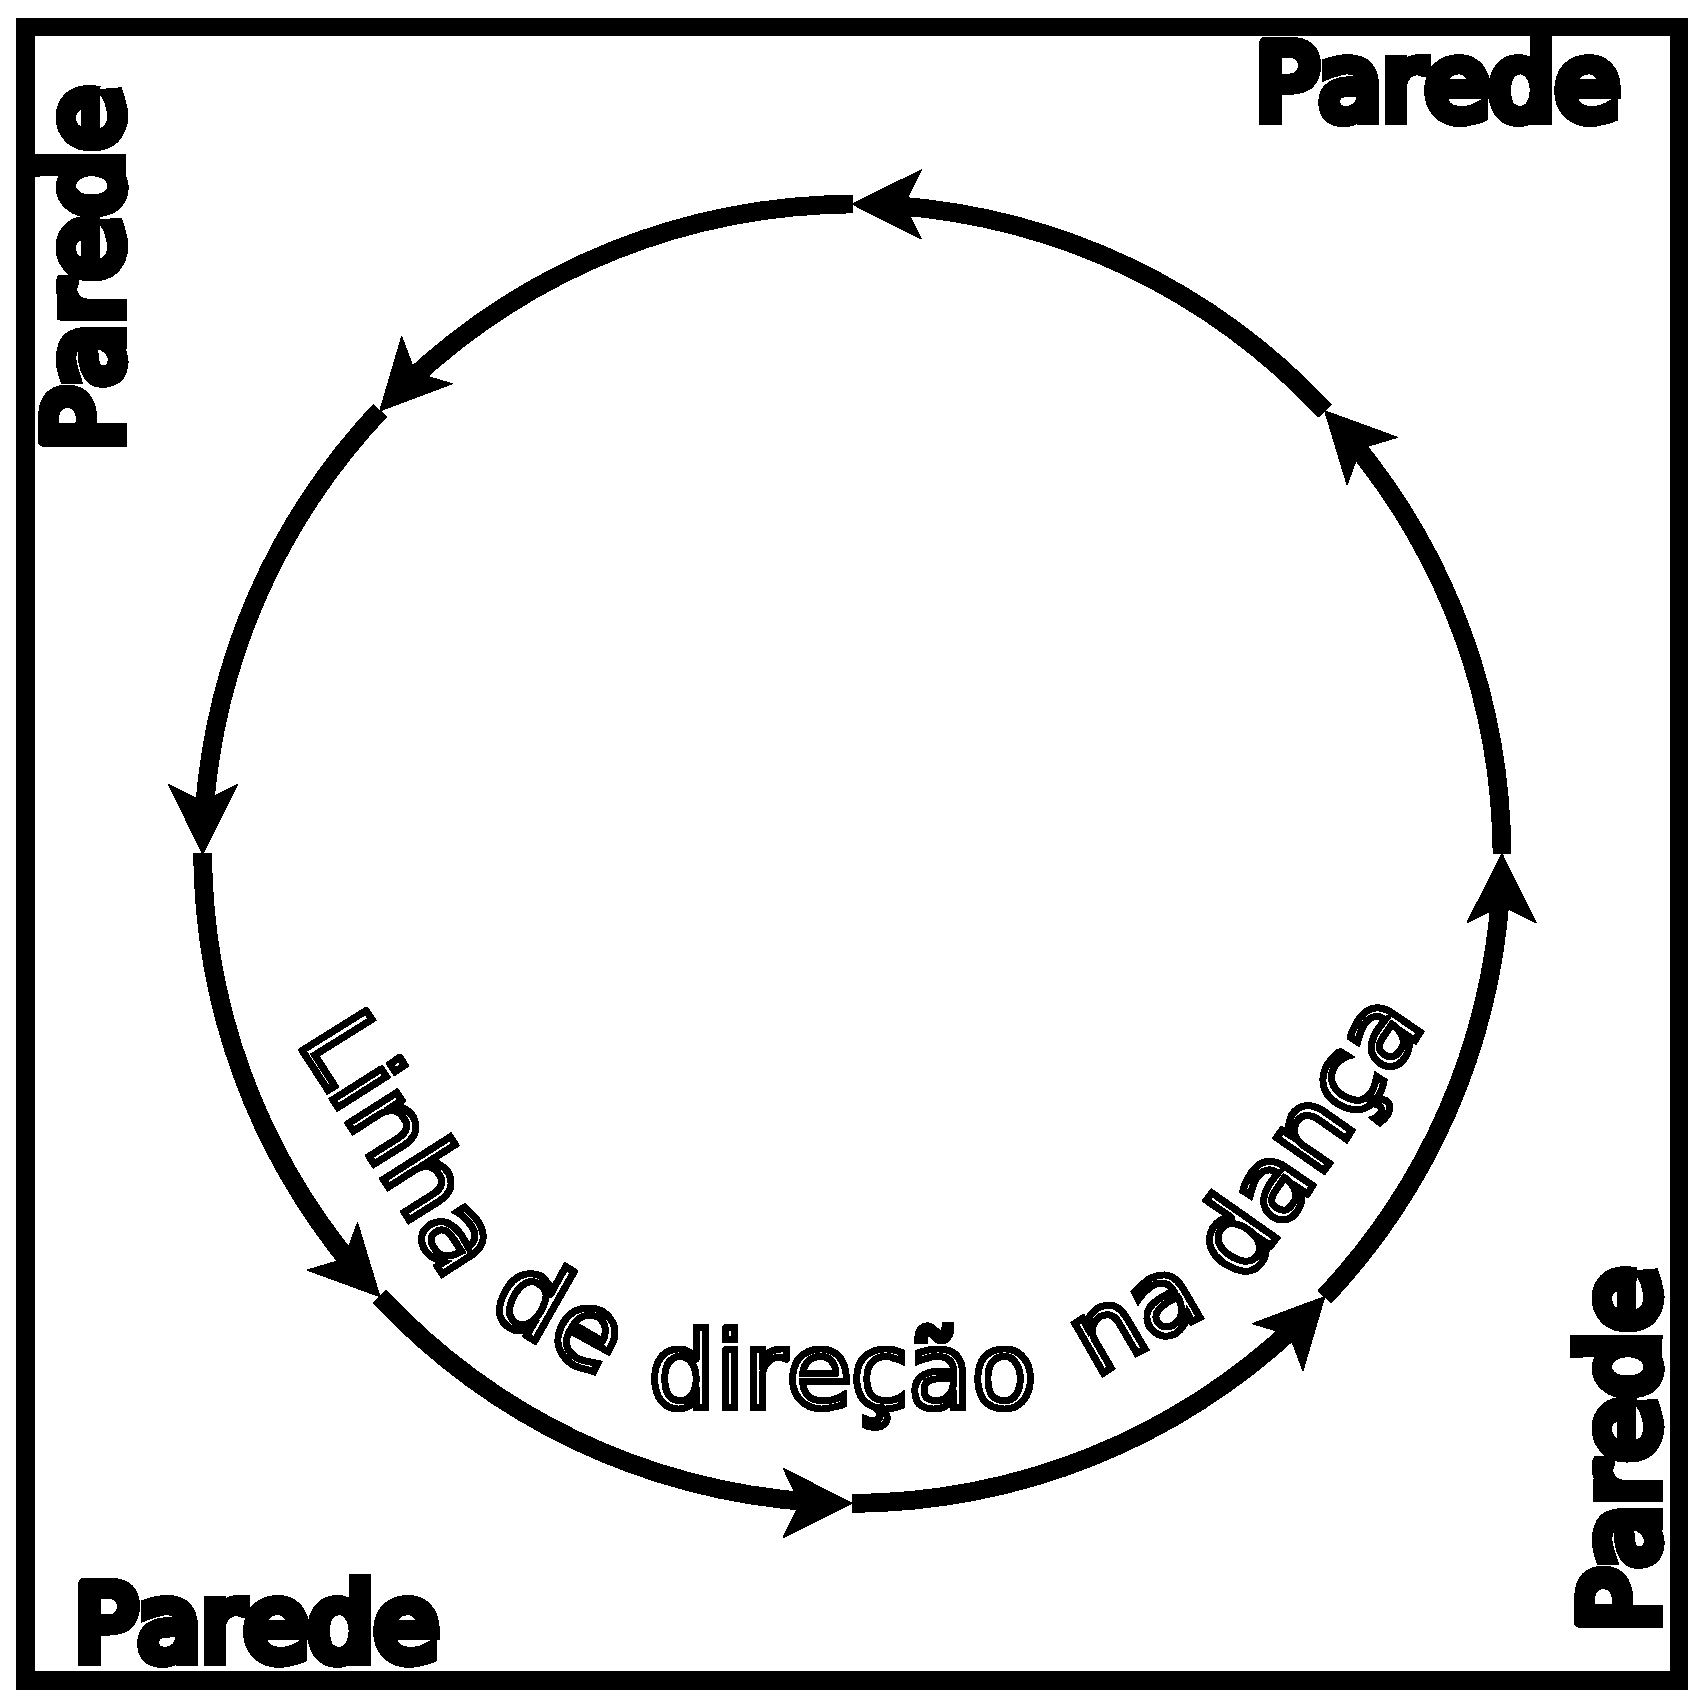
\includegraphics[width=0.3\textwidth]{chapters/cap-normas/circular-antihorario.eps}
\caption{Linha de direção nas danças com  deslocamento circular \cite[pp. 20]{freitas1959danca}.}
\label{fig:giro-antihorario1}
\end{figure}
Visto o anterior é importante ressaltar que né todas as danças tem
uma evolução circular na pista de dança, pois existem estilos de dança que são dançados em linha,
como por exemplo a ``Salsa em linha'' ou o ``West coast swing''; ou também existem estilos que
tem um comportamento hibrido entre circular e linha como o "Zouk". Neste sentido,
a ``samba de gafieira'' tem um comportamento circular e  deve ser dançado
rodando o salão para um boa etiqueta na pista de dança.


\item[Conduzir e ser conduzidos:] Trabalhar num \hyperref[def:ParadigmaConducao]{\textbf{paradigma da dança baseado
na condução}} é muito importante para na \hyperref[def:DancaSalao]{\textbf{dança de salão}}, dado que isto implicará
que um \hyperref[def:Condutor]{\textbf{condutor}} habilidoso, poderá dançar fluidamente com pessoas com quem nunca dançou
antes (se esta for conduzível). De forma similar acontecerá para os \hyperref[def:Seguidor]{\textbf{seguidores}} que desenvolvam
a sensibilidade necessária para serem conduzíveis, elas poderão dançar com qualquer
condutor, inclusive poderão ter um desenvolvimento básico em estilos de dança pouco ou não conhecidos.

O caso oposto ao \hyperref[def:ParadigmaConducao]{\textbf{paradigma da condução}}, é ter um estilo de dança baseado em coreografias;
este enfoque, dependendo da finalidade, pode ser visto como um vicio que geralmente aparece quando iniciamos
na dança. 
\begin{example}
Quando a pessoa que deve conduzir, assume que se esta realiza a parte do movimento 
que lhe corresponde, sem enviar nenhuma informação ao \hyperref[def:Par]{\textbf{par}}, 
então o \hyperref[def:Seguidor]{\textbf{seguidor}} deve reconhecer/adivinhar e realizar o movimento que o condutor imaginou.
\end{example} 
O enfoque do exemplo anterior, funciona bem quando ambos dançarinos tem treinado antecipadamente os movimentos, 
e/ou conhecem a sequencia em que estes movimentos serão executados; 
porem, falha quando os dançarinos não se conhecem.
Comprovar isto é fácil se imaginamos, por exemplo, o caso em que o \hyperref[def:Condutor]{\textbf{condutor}} executa um movimento
que tem a parte inicial muito parecida a outro movimento, nesse caso, se o \hyperref[def:Seguidor]{\textbf{seguidor}} não tiver
um poder telepático confundirá um movimento com o outro e acontecerá um problema de comunicação. Assim, a coreografia
na dança deve estar reservada para apresentações, onde o \hyperref[def:Par]{\textbf{par}} volta 
a sua atenção para a encenação da peça, e não para detalhes mais mecânicos.

\item[Peso do corpo definido num pé:] Em estilos de dança onde uma boa postura é requerida,
ter o peso total do corpo bem definido sobre um pé, 
ao final de cada ação ou proposta de movimento,
quando sabemos que realizaremos mais movimentos imediatamente depois;
garante conservar a postura e ter uma maior velocidade no tempo de reação para o seguinte movimento;
pois, ao ter um pé livre poderemos mover ele sem temor a perder o equilibro, 
o que se traduz na leveza na execução dos movimentos. 
Isto é facilmente comprovável se fazemos um pequeno exercício. 
\begin{example}
Ao ficar em pé separamos as
pernas uma distancia igual à de nosso quadril, e nesse momento levamos o peso do corpo\footnote{
Em física podemos representar um corpo como um objeto com a masa concentrada no seu centro de gravidade, 
que no casso do ser humano está perto do umbigo.} a
apontar a um ponto médio entre nossos pés, nesse instante estamos dividindo o peso do corpo
entre nossos dois pontos de apoio, 50$\%$ no pé direito e 50$\%$ no pé esquerdo; agora, mantendo o peso
do corpo nesse lugar, tentaremos levantar qualquer de nossos pés, será evidente
que esse trabalho é muito difícil sem perder o equilíbrio, pois para mantê-lo
precisamos de ambos pontos de apoio; casos similares podem ser vistos com qualquer proporção de distribuição de peso,
por exemplo, 30$\%$ e 70$\%$ ou 20$\%$ e 80$\%$. 
\end{example}
Assim, do exemplo anterior se deduz, que estaremos
equilibrados, e poderemos executar nossos movimentos e levantar um pé 
mantendo a postura e auto controle, quando
temos o 100$\%$ do peso do corpo num pé só, o pé de apoio.
 
Por outro lado, quando consideramos ao 
\hyperref[def:Condutor]{\textbf{condutor}} como o agente desequilibrante do \hyperref[def:Seguidor]{\textbf{seguidor}}, 
por exemplo no caso em que este aplica uma condução;
a ideia de manter o peso do corpo num pé só, tem um valor agregado; 
pois fica mais fácil para o condutor orientar
ao seguidor a fazer o seguinte movimento, dado que o único pé que o seguidor pode mover é o pé
que está livre, e que é o pé que o condutor precisa que se movimente, 
além de que a força necessária pelo condutor para tirar ao seguidor do seu equilíbrio 
atual é muito menor ao caso quando o seguidor tem dois pontos de apoio.
Adicionalmente o seguidor tem um pé livre para se resguardar do desequilíbrio, provocado pelo 
condutor, e adquirir um novo equilíbrio com esse pé.

Outra forma equivalente de descrever, a localização do peso do corpo, 
é indicar que o peso do corpo deve recair sobre o pé que está em frente, 
quando realizamos um passo de avanço, 
e no pé que está atrás quando realizamos passos de recuo \cite[pp. 19]{freitas1959danca}.


\textbf{Nunca podemos dividir o peso do corpo?} Esta caraterística é possível sim,
se nossa dança fosse um relato escrito, o peso de nosso corpo deve estar bem definido num pé,
ao final de cada palavra, em cada virgula e ponto e virgula; por outra lado, 
o peso do corpo pode estar dividido em cada ponto.

\textbf{Este é o único meio de manter o equilíbrio na dança?}  Não, 
existem estilos de dança, como por exemplo no ``lindy hop'' onde se consegue manter os pês libres, 
para executar os movimentos, mantendo um equilíbrio dinâmico,
realizando um movimento de rebote (chamado ``bouncing'') ao ritmo da música.
O movimento consiste em deixar cair nosso corpo, flexionando ligeiramente  os joelhos, 
e imediatamente volver a ficar em pé, realizando assim um efeito de mola. 

\item[Ter uma boa conexão entre o par na dança:] Seguindo a ideia da condução, esta só pode
ser realizada se existe um médio de comunicação, onde possa ser transmitido
o comando do \hyperref[def:Condutor]{\textbf{condutor}} ao \hyperref[def:Seguidor]{\textbf{seguidor}}. 
Assim, um boa conexão garante este fluxo de informação entre o \hyperref[def:Par]{\textbf{par}} na dança. 
A forma exata de obter esta conexão varia ligeiramente entre os diferentes estilos de dança;
dado que em alguns casos será usado um \hyperref[def:abracodedanca]{\textbf{abraço de dança}} 
e em outros o par estará conectado segurando-se das mãos.
Mas, em todos os casos, 
o que se procurará é ter a maior quantidade de pontos de contato no par,
pois quanto mais pontos de contato tenhamos, 
maior será a fidelidade com que a informação da condução chegue ao seguidor.


Outro ponto importante desta conexão é a \hyperref[def:brazosfirmes]{\textbf{firmeza dos braços}}, 
pois é a traves deles que passa a maior parte da informação.
Assim, no caso do seguidor, ter os braços firmes implicará que qualquer informação que chegue por eles,
se transmitirá maioritariamente ao corpo,
mudando assim este de estado ou posição.

Em estilos de dança onde existe a possibilidade de dançar tomados das mãos,
se não se tem bem treinados os braços,
é muito fácil que a informação da condução seja perdida.
Isto acontece, porque no braço todo, temos vários graus de liberdade nas articulações.
Se algum destes pontos não tem a firmeza necessária para transportar a informação de condução, 
sem modificar maioritariamente sua posição relativa e postura,  
então esse ponto provocará a perdida da informação, 
pois se modificará a posição dos braços sem alterar a posição do corpo.
\begin{example}
De pie frente a frente com seu par, testaremos 3 tipos de condução, 
criadas quando o condutor segura com as mãos ao seguidor, em 3 lugares diferentes:
\begin{itemize}
\item Segurando num ponto meio entre entre o cotovelo e os ombros,
\item segurando no antebraço, e
\item tomados das mãos.
\end{itemize}
\end{example}
No exemplo anterior, será muito evidente em seguidores iniciantes,
que a maior eficacia na transmissão de informação se consegue segurando entre os cotovelos e os ombros,
seguido por segurar pelo antebraço, e finalmente nas mãos;
é dizer, a eficacia na transmissão da informação, 
diminuí com o aumento dos grãos de liberdade.

Assim, para obter uma boa conexão no par, 
e eficacia na transmissão de informação, devemos ter:
\begin{itemize}
\item Uma boa postura de braços e
\item procurar a maior quantidade de pontos de contato.
\end{itemize}  

\end{description}

%%%%%%%%%%%%%%%%%%%%%%%%%%%%%%%%%%%%%%%%%%%%%%%%%%%%%%%%%%%%%%%%%%%%%%%%%%%%%%%%
\section{Princípios elementares no samba de gafieira}
\label{sec:principiosambagafieira}
\index{Princípios elementares!Samba de gafieira}

É evidente olhando aos profissionais da dança,
que cada pessoa tem uma forma particular de dançar, 
que carateriza e identifica a ela. Porem, 
dentro desse margem pessoal de trabalho, 
pode ser identificado que a pessoa está realizado um estilo de dança em particular,
por exemplo: samba de gafieira, forró, salsa, etc.
Assim, se conclui que existe um conjunto de caraterísticas na dança,
que provocam que estas sejam enquadradas num estilo particular;
estas caraterísticas não são todo ou nada, é dizer, 
não precisam cumprir-se todas para reconhecer um estilo de dança,
porem, quanto maior sejam as caraterísticas usadas mais fácil será enquadrar uma dança num estilo de dança em particular.

Os princípios elementares planteadas aqui, são uma tentativa de enumerar as caraterísticas,
que tenho observado, que provocam que um espectador ou dançarino,
vejam ou percebam que se está dançando samba de gafieira.
\begin{description}
\item[Quadril avança, ombros e pé acompanham:]  Os movimentos, no samba de gafieira, 
que pretendem evocar uma estética relacionada com a malandragem,  geralmente iniciam no quadril;
isto provocará que as demais partes do corpo (pernas e torço) atuem a consequência para achar um novo equilíbrio.
Adicionalmente ajudará a que ao terminar o movimento, o peso de nosso corpo esteja imediatamente bem posicionado sobre um pé só.
Porem esta caraterística é só interessante, 
se o que o dançarino está procurando são elementos que contribuam a uma estética de malandragem;
para estéticas mais estilizadas, suaves e menos abruptas devemos estudar os modos de transferência do peso do corpo.

%\item[Pisar com 100$\%$ do peso do corpo:] %quando se movimenta um pé.
\item[Transferência do peso do corpo:] %quando se movimenta um pé.
Uma característica do samba de gafieira é uma estética que evoca à malandragem, 
uma forma de contribuir para obter esta estética é que ao movimentar um pé, 
este ao tocar o chão chegue com o 100\% do peso do corpo; realizar esta ação é fácil, 
se temos cumprido que nosso movimento inicie desde o quadril e não por esticar as pernas.

Assim, existe uma diferença com outros estilos de dança, 
como o bolero e o tango, 
onde se procura projetar uma estética de elegância e com movimentos fluidos;
nestes estilos, no movimento de pés, primeiro se aponta com a ponta do pé sem levar o peso do corpo,
 e logo o peso é transferido ao lugar apontado, numa dinâmica continua de aponta e transfere,
criando essa estética elegância e fluides ao se deslocar.

Isto \textbf{não} quer dizer que a dinâmica de aponta e transfere seja menos interessante e não possa ser usada no samba de gafieira,
e sim que o dançarino deve escolher que imagem deseja projetar em cada momento,
malandragem, elegância ou misturas intermédias, e para isto deve escolher o jeito de como vai transferir o peso do corpo. 

Um paralelismo com a música, pode ser feito com o estudo da transferência de peso na dança;
no caso da música existem símbolos de \hyperref[sub:Articulation]{\textbf{articulação}}, 
que indicam como as notas musicais devem ser executadas e articuladas entre sim;
por exemplo temos símbolos como: legato, staccato e tenuto;
que indicam que a articulação dos tons entre as notas musicais consecutivas deve ser: fluida, ressaltada e  abrupta, respetivamente.
Pelo que se queremos ser coerentes com a música, 
ou da porção dela que desejemos interpretar,
deveríamos escolher cuidadosamente nosso modo de transferência de peso.


\item[Ter um bom abraço no samba de gafieira:] Como já foi mencionado na Seção \ref{sec:PrincipioGeral}, 
ter uma boa conexão na dança é muito importante para uma boa transferência de informação na condução; 
porem, existem particularidades desta conexão na samba de gafieira que devem ser ressaltadas.

Por exemplo, na maioria de movimentos se usa o \hyperref[def:abracodedanca]{\textbf{abraço de dança}};
mas, particularmente em samba de gafieira, se precisa que o braço esquerdo da dama tenha contato
e rodeie, pela parte externa, ao braço direito do condutor; 
de modo  que o seguidor não se debruce sobre o condutor,
e sim que mantenha um atrito entre os braços.
A importância deste contato radica em que o condutor em algumas situações precisam transmitir conduções, 
que provoquem a sacada de perna do seguidor (ex: Edmundo, sacadas, etc.), 
e isto é transmitido realizando o condutor um movimento de rotação do tórax no plano axial.  
Rotando em sentido horário para tirar a perna direita do seguidor, 
e em sentido anti-horário para tirar a perna esquerda do seguidor;
é neste ponto que esse atrito entre os braços é importante, 
pois quando se realiza o movimento de rotação anti-horário, se não existisse o atrito,
o tórax do condutor giraria só, sem afetar o tórax do seguidor ou afetando muito pouco;
assim, o atrito garante que esta informação na torção chegue com maior eficacia ao seguidor,
ver Figura \ref{fig:torcao-abraco}.
\begin{figure}[h]
  \centering
    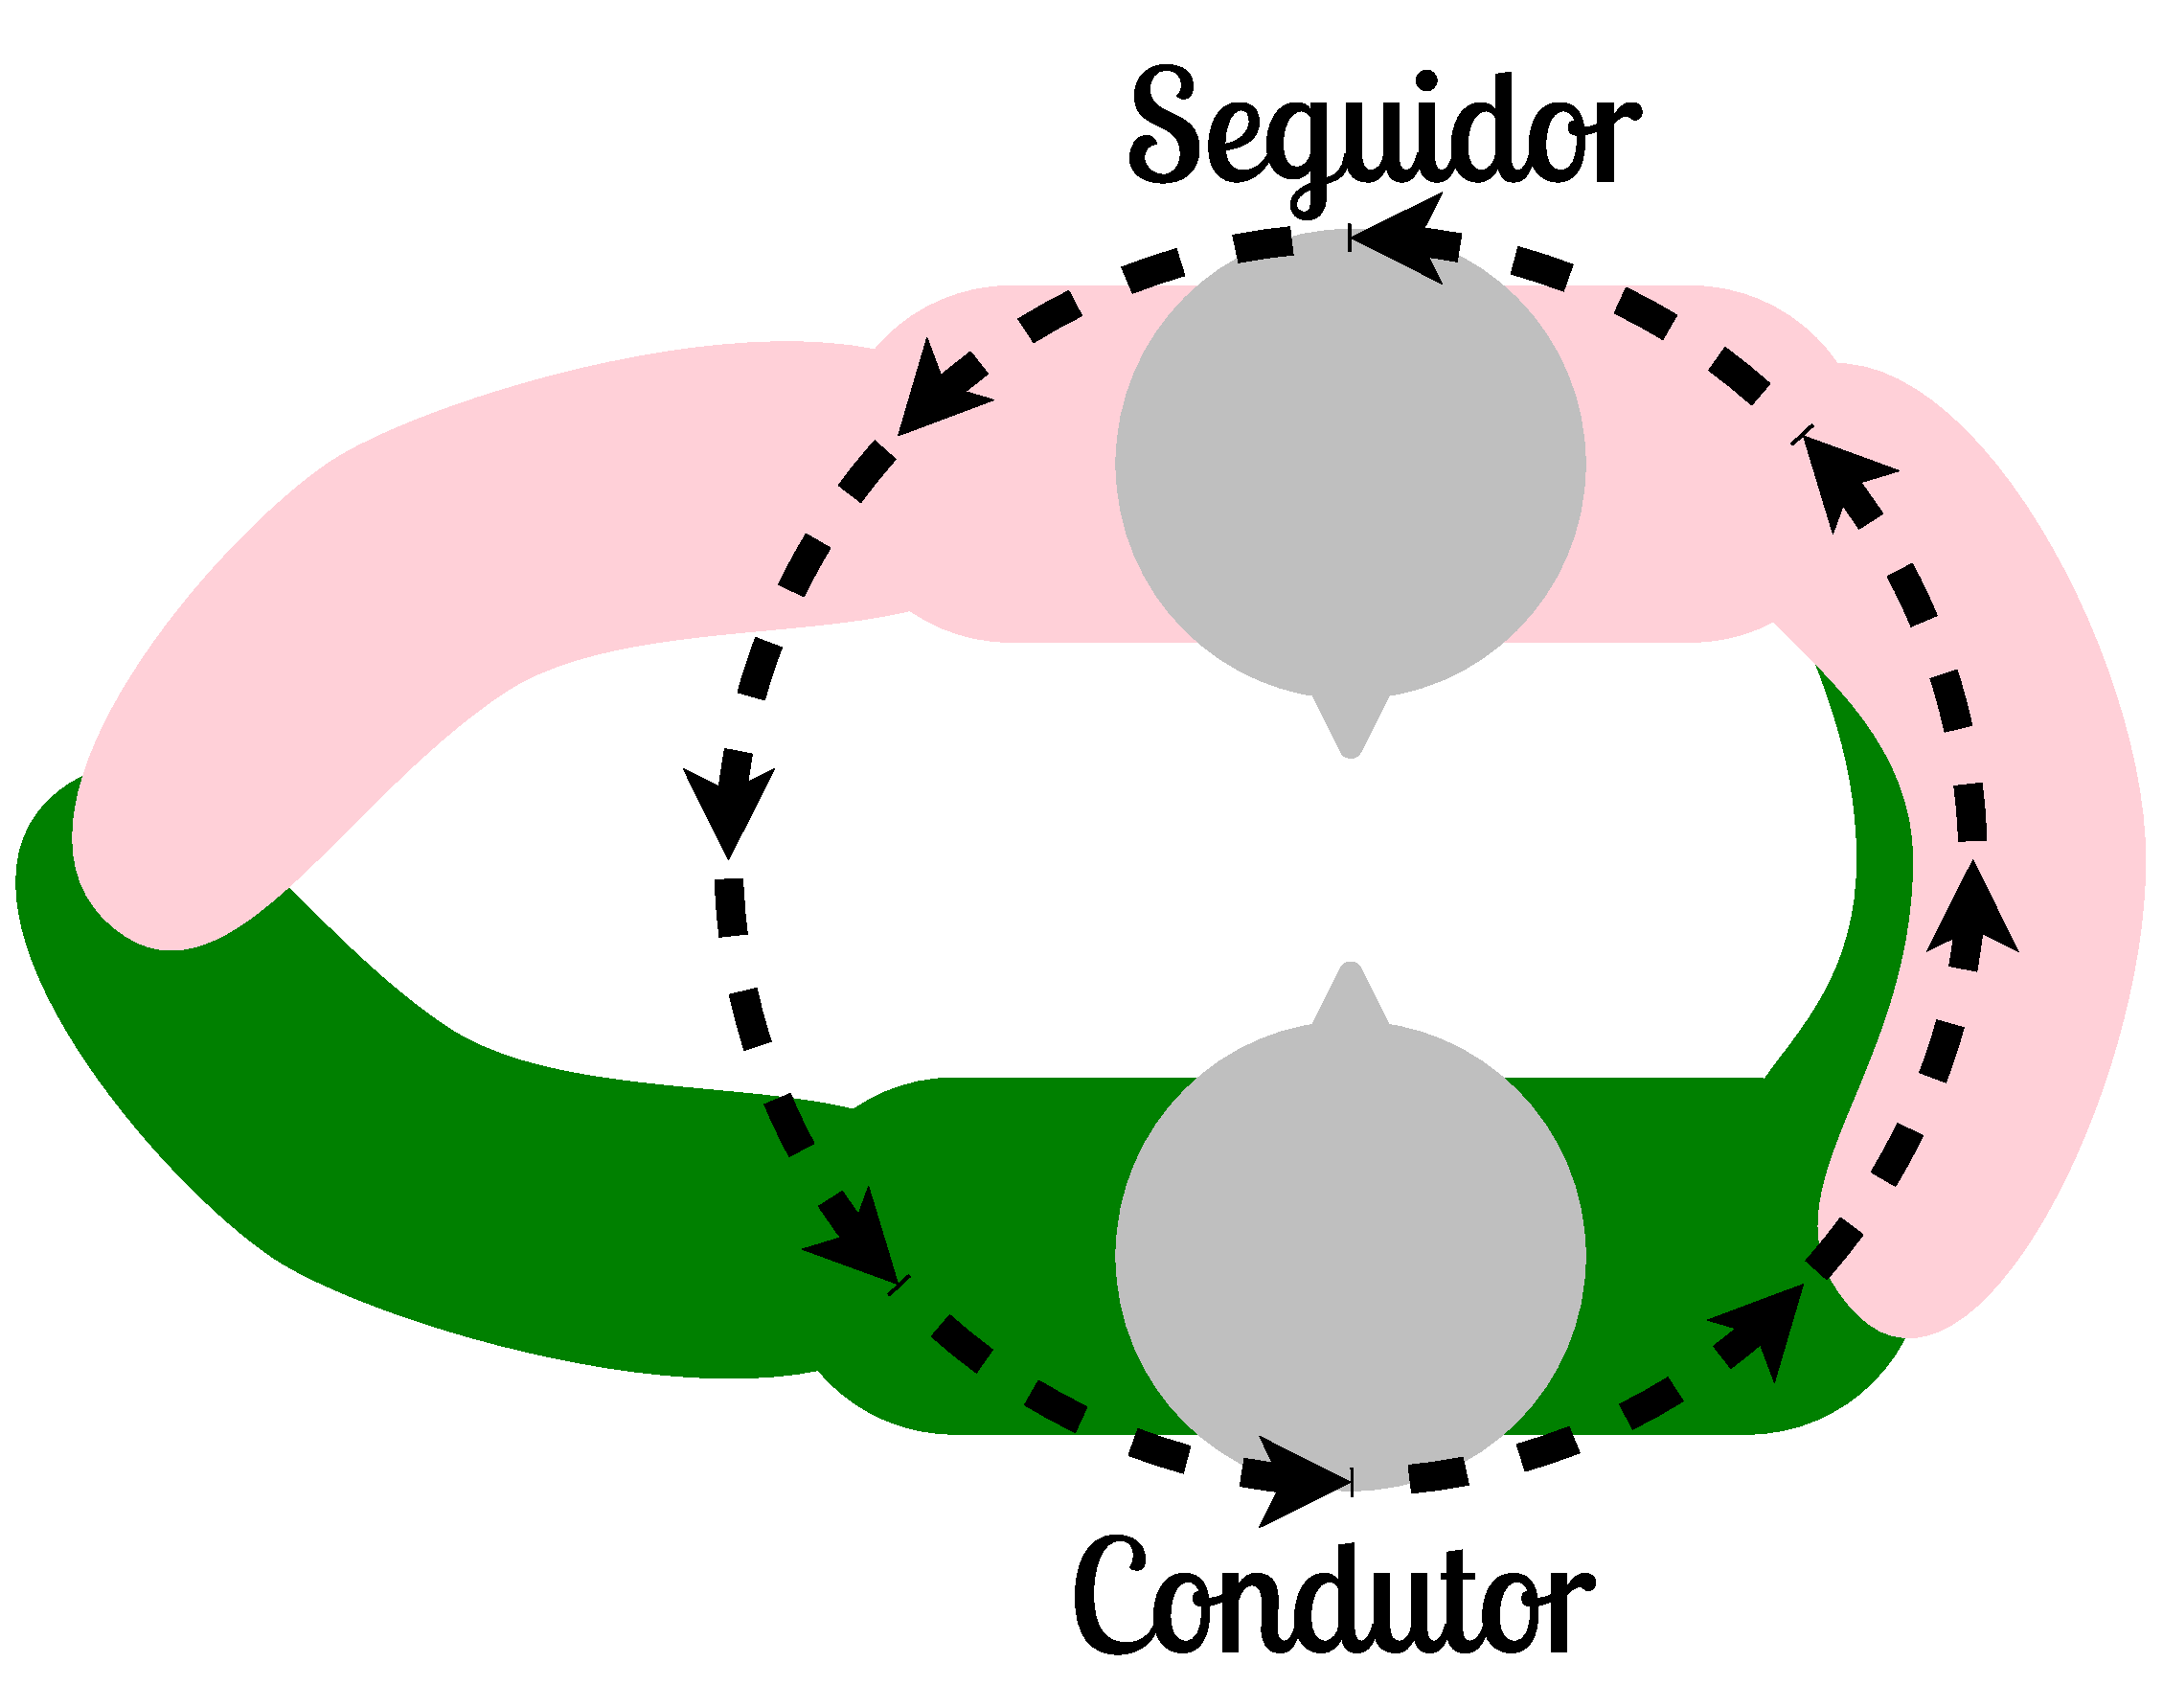
\includegraphics[width=0.4\textwidth]{chapters/cap-normas/torcao-abraco.eps}
\caption{Transferência de informação de condução ao seguidor, mediante do torção do tórax no sentido anti-horário.}
\label{fig:torcao-abraco}
\end{figure}

Por outro lado, em alguns momentos na dança, de samba de gafieira, usaremos um abraço de dança mais separado,
para realizar passos como o ``picadilho''; em estas circunstancias, é o braço direito do seguidor,
que precisa em todo momento estar \hyperref[def:brazosfirmes]{\textbf{firme}}, 
mantendo uma ativação muscular e diminuição dos graus de liberdade,
para que toda a informação enviada pelo condutor atravesse os braços e o tórax do seguidor,
e chegue sem degradação ate o quadril, onde se provocará a movimentação de pés planejada pelo condutor.

\item[Abraço uniforme do condutor:] Continuando com as particularidades do abraço,
mas agora no âmbito da distancia de separação entre o \hyperref[def:Par]{\textbf{par}} durante o tempo que dure o abraço.
É importante ressaltar que deves-se manter uma regularidade na distancia de separação,
e evitar um ``abraço sanfona'', é dizer um abraço onde o condutor as vesses, 
aperta demais ao seguidor, e outras vesses onde deixe ele solto e mais separado dele.
É claro que esta irregularidade do abraço, existe na dança; 
mas, esta deve ser uma coisa consciente e projetada 
pelo condutor em função da técnica necessária para realizar um passo; 
e em nenhum caso deve ser uma coisa  fora de controle ``sanfonando'' ao par.

Um momento onde é altamente importante esta regularidade, 
é durante passos como ``gancho redondo''.
Por outro lado, termos momentos em que precisaremos ajustar a distancia do abraço,
antes do inicio do passo, para mais perto no caso do ``pião'' e para mais longe no caso do ``picadilho''.

\item[Procurar o paralelismo de ombros no par:] 
Um ponto muito cobrado, na dança de salão é manter a linha de visão no \hyperref[def:Par]{\textbf{par}},
em samba de gafieira esta caraterística é obtida mantendo sempre paralelas, as linhas dos ombros, no par.
Isto além de um ganho estético, tem interessantes caraterísticas técnicas;
pois se a combinamos com a ideia de manter sempre a mesma distancia no par;
chegamos a um ponto onde poderemos estabelecer uma condução por indução, ou condução sem contato.

A responsabilidade de manter este paralelismo de ombros é do \hyperref[def:Seguidor]{\textbf{seguidor}},
pois este deve ``seguir'' o movimento do \hyperref[def:Condutor]{\textbf{condutor}}.
Por outro lado o condutor tem a responsabilidade de realizar os movimentos com uma velocidade e clareza necessárias, 
para que estes possam ser acompanhados pelo seguidor.

\item[Conduzir pelo tórax não pelos braços:] 
Se conseguimos ter paralelismo na linha dos ombros,
e se procuramos manter sempre a mesma distancia, 
e linha de visão com o \hyperref[def:Par]{\textbf{par}}, 
sem a necessidade do uso dos braços;
pode-se deduzir que, nestas dinâmicas corporais,
é o tórax do \hyperref[def:Condutor]{\textbf{condutor}} quem guia ao \hyperref[def:Seguidor]{\textbf{seguidor}}.
Isto implica que os braços tem o papel de brindar sustento para a transferência de informação da condução,
porem os braços do condutor, não são os executantes e protagonistas da condução;
sendo, principalmente o tórax do condutor, a fonte mecânica desta informação.
Este dado é muito relevante em passos como o ``Romário'' ou o ``gancho redondo'',
onde é o tórax, e não os braços, do condutor que leva ao seguidor de um lado a outro. 

\item[O pé de apoio deve apontar ao par:] 
Quando nos encontremos numa postura, em que o peso do corpo está definido totalmente num pé;  
é dizer, quando não estejamos num movimento de transferência de peso;
o pé que contem o peso do corpo debe apontar a um ponto médio entre os pés do \hyperref[def:Par]{\textbf{par}} de dança.
Esta caraterística tem um proposito além de estético, técnico;
dado que o corpo tende a ir em direção a onde esta apontando nosso pé,
assim ao apontar sempre ao par, 
garantimos que em todo momento procuraremos a proximidade e teremos uma linha de visão  com ele.
Uma boa metáfora, é pesar que a ponta de nosso pé é uma bússola que aponte ao norte que é nosso par.
\end{description}
